% 

\documentclass[10pt,a4]{article}

\usepackage{cogsci}
\usepackage{pslatex}
\usepackage{apacite}
\usepackage{graphicx}
\usepackage{csquotes}
\usepackage{tipa}


\title{Influences of Uncertainty Optimization on the Development of Language}
 
\author{{\large \bf Christopher Dilley} \\
	 christopher.dilley@student.uni-tuebingen.de \\\And
	{\large \bf Erik Schill} \\
	email@email.com \And
	{\large \bf Inna Pirina} \\
	email@email.com }


\begin{document}

\maketitle


\begin{abstract}
	
	Determining the ancestry and relationship of languages is one of the primary challenges that historical linguists face.  The task is daunting and tedious, and is prone to the subjectivity of the researcher.  For these reasons, it has been of great interest to develop means of automating the process.  In this paper, we discuss a reimplementation of one such process, which builds a representation of the internal structure of a language to compare against those of other languages and establish a measure of their relatedness.
	
\end{abstract}


\section{Background}

This paper aims to determine the linguistic relatedness of a number of languages in the same manner as described in \citeA{ellison2006measuring}, using an improved dataset.  

When linguists perform the task of building phylogenic tree, they typically do so by comparing cognates between languages, and reconstructing their forms in a shared proto-language.  Some attempts at automation build upon this idea, comparing words of the same meaning across languages and judging their similarity and potential cognacy.  The approach used here instead compares words within a language in order to avoid issues of languages using different orthography or having different phonetic spaces.

Kirby and Ellison describe a process whereby a language is quantified as a matrix comparing the probability of confusing one word for another for every word pair in the language, and these matrices are compared and clustered based on their relatedness.  By doing so, they achieved very encouraging results, automatically generating a phylogenic tree of languages that closely resembles the generally accepted phylogeny; nearly all of the languages fell neatly into their respective language subfamilies.

In employing a new set of data, we hoped to obtain equal or better results.  This new data set contains more data than that used by the authors in the paper, and uses each word's phonemic transcription rather than its orthography to calculate confusion probabilities.  We hypothesized that the language's phonemics would expose more meaningful relationships between words than orthography, as orthography can vary widely.  For example, the English words 'though' and 'toe' have significantly different orthography, while being pronounced very similarly (\textipa{[Do:]} and \textipa{[to:]}).

However, it is possible that this may give worse results as well.  Orthography may better represent the ancestry and relatedness of individual words, even when their phonetics converge.  The fact that 'though' and 'toe' are pronounced similarly may simply be due to random sound shifts causing phonetic convergence by chance, and this phonetic similarity may lead measures of word interrelatedness astray, negatively affecting intra-language comparisons. 

This study seeks to identify which of these hypotheses is more likely. \\

\textbf{- PHONETICS vs. PHONEMICS vs. PHONOLOGY... WHICH IS CORRECT USAGE HERE?}

\section{Implementation}

Our methodology follows much of the same procedures as \citeA{ellison2006measuring}.  We developed our own tools for generating the lexical metrics of all languages and for comparing them as well, while using an external tool to render the phylogenic trees from the resulting data.

As our input, we obtained data from the Indo-European Lexical Cognacy Database.  This data set spans 208 word meanings across 52 languages (not all languages had data for all word meanings), and includes phonemic transcriptions for all words.  We used these transcriptions instead of the word orthography for the inter-lexical comparisons, expecting to better detect similarity between words.\\

\textbf{- PROBABLY WANT TO CITE THIS DATABASE, BUT I COULDN'T FIND A GOOD WAY TO DO SO... AND NO OTHER PAPERS THAT USE IT SEEM TO CITE IT}\\

\subsection{Calculating Lexical Metrics}

(Talk about this process of comparing all words inside each language to generate the matrices)

Hey, look at the lexical metric in Figure~\ref{fig:french}.

\begin{figure}[ht]
\centering
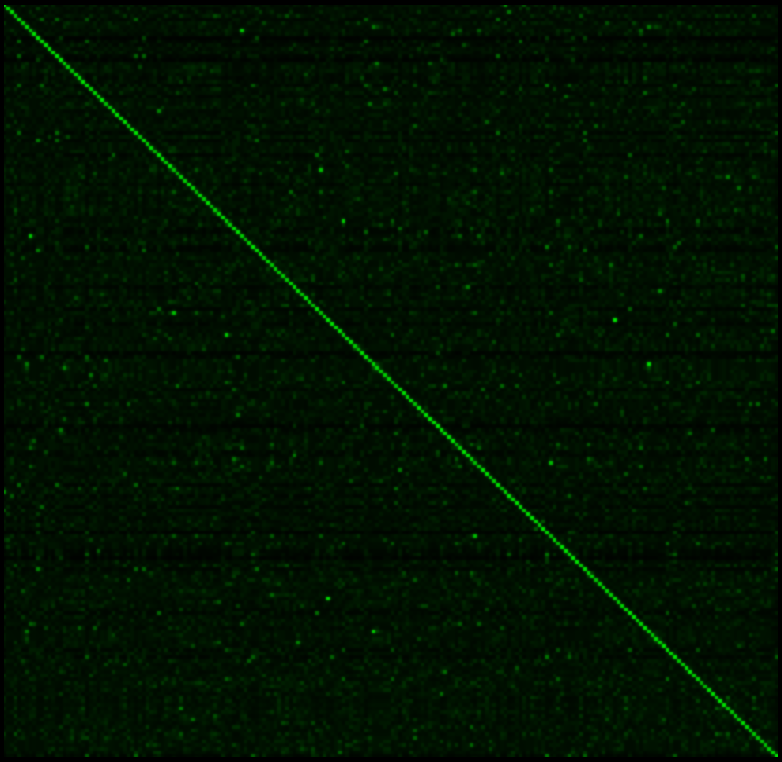
\includegraphics[width=0.8\linewidth]{french3}
\caption{A visualization of the lexical metric for French.}
\label{fig:french}
\end{figure}



\subsection{Calculating Language Distance}

Once we have constructed the lexical metrics for each of the 52 languages in our corpus, we could apply the methods described in the Section 3 of the Kirby and Ellison paper. 

Before computing the distances between the languages, however, we had to ensure that all of the language matrices were consistent. That implied that in each of the languages’ matrices, the rows and columns should correspond to the same meanings; this proved to be slightly problematic. 

Firstly, we found, that in the corpus we were working with, there were very few meanings that were shared by all of the languages. That led us to the decision of constructing large matrices (for all 208 meanings), but completely ignoring the values of the meanings that were not present in a language. 

Secondly, some of the languages contained multiple forms for one meaning, while others did not. That raised a question of which of the several present forms we should choose to include to the language’s matrix. After some discussion, our final solution was to only take the form with the greatest sum of probabilities.  We argue that this makes the most sense, as word with higher confusion probabilities means that it is more similar to other words in the language, and may better represent the lexical structure of the language.  However, this decision was arbitrary, and other methods could instead be used, such as using the minimum or the average.

The authors argued that in order to compare two languages, one should compute the distance between them. Since all of the languages were already represented as probability distributions (matrices), the distance between two matrices could be calculated. There were two types of distance calculations used in the paper, computed using the language matrices: Kullback-Liebler (KL) distance and Rao distance. Both distances are commonly used by statisticians to measure the divergence of two probability distributions.  The formulas and their application to the data is explained in greater detail by \citeA{ellison2006measuring}.

Calculating the KL distance and Rao distance for a pair of languages involved comparing all of the elements of both matrices for which both languages had word meaning data. The script for implementing the formulas was written in Python. 

Having compared the matrices of two languages using both KL and Rao distances, we obtained a numerical distance value for each of these methods. We then repeated the process for each pair of the languages in the data set and got the distance measures for each pair. These values were then assembled into another matrix, where the rows and columns represent each language, and the values represent the distance between the row's and the column's languages. In the end, we had two of such matrices: one containing the KL distances for all language pairs, and another containing the Rao distances.

\textbf{- I'VE ADDED THE ORIGIN PAPERS FOR KL DISTANCE AND RAO DISTANCE TO THE BIBTEX FILE, BUT WE PROBABLY DON'T NEED TO CITE THEM RIGHT?  SINCE WE PULLED THEM FROM THE MAIN PAPER?}

\subsection{Constructing Phylogenic Trees}

Once having constructed a matrix that represents the distance between all language pairs in the collection, these results need to be converted into an analyzable form.  Specifically, we want to visualize how close certain language pairs are related, and how they cluster together into larger groups.  From this, we hope to see some of the same taxonomic relations that are generally accepted as language families and subfamilies.

In order to accomplish this, we began by using the \textit{NEIGHBOR} program from the \textit{PHYLIP} package \cite{web:phylip}, as was done in the paper.  This program takes a matrix input, and constructs a tree that represents the relatedness of all of the languages based on their distance measurement.  This tree is output in a text form (in the standardized 'Newick' format) that describes the nodes on the tree and the distance to their child nodes.  Once having generated this, we used the Phylodendron tool from the University of Indiana to visualize this information as a proper tree \cite{web:phylodendron}.  

This process was repeated separately for both the KL distance matrix and the Rao distance matrix.

\section{Results}
	
The results from using Kullback-Liebler distance are found in Figure~\ref{fig:kltree}, and the results from using Rao distance are found in Figure~\ref{fig:raotree}.

In our results, it can be seen that the algorithm does a good job of grouping similar languages together in the tree.  Well-accepted subfamilies of languages can be seen together.  The Rao distance tree seems to do a better job of this grouping, seeing more definable groups with greater consistency.

Some outliers are evident in this tree.  Danish, Norwegian, and Swedish find themselves far separated from their closely related Scandinavian languages (Faroese, Icelandic, etc.), and other Germanic languages (German, English, Dutch) are not grouped well with them at all.  French and Catalan are also similarly separated from their other Romance counterparts (Latin, Spanish, Italian).

Outside of these outliers, the groupings seems quite sensible.  Indo-Iranian languages (Urdo, Ossetic, etc.), Slavic languages (Russian, Czech, Polish, etc.), and most of the Romance languages (Spanish, Italian, etc.) are seen grouped together.  However, the combining of these smaller groupings into larger groupings seems to not make as much sense.

	
\begin{figure*}[ht] 
	\centering 
	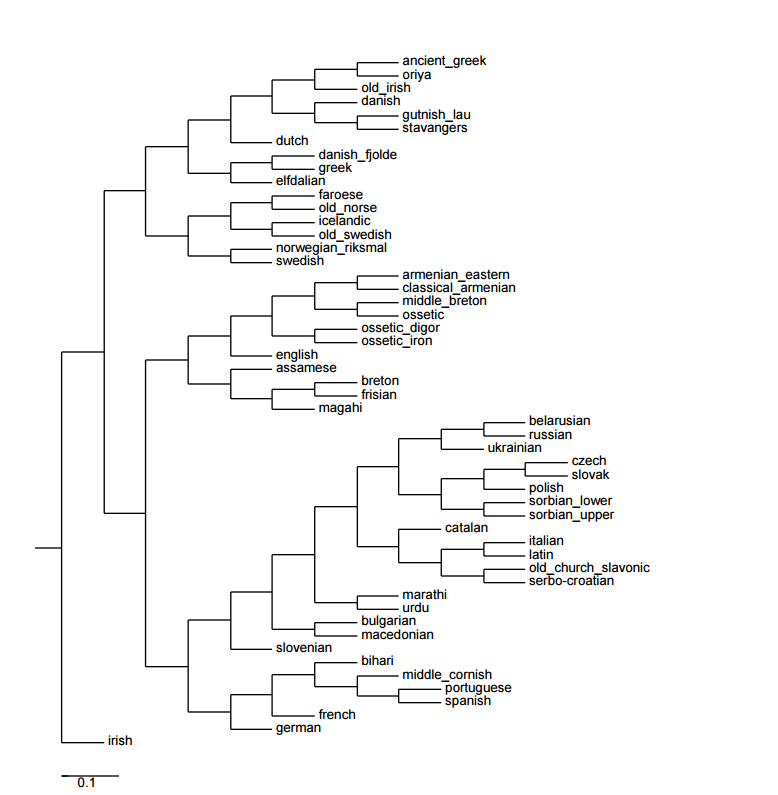
\includegraphics[width=\linewidth]{tree1(3)}
	\caption{Tree visualization of KL-distance measurements}
	\label{fig:kltree}
\end{figure*}

\begin{figure*}[ht]
	\centering
	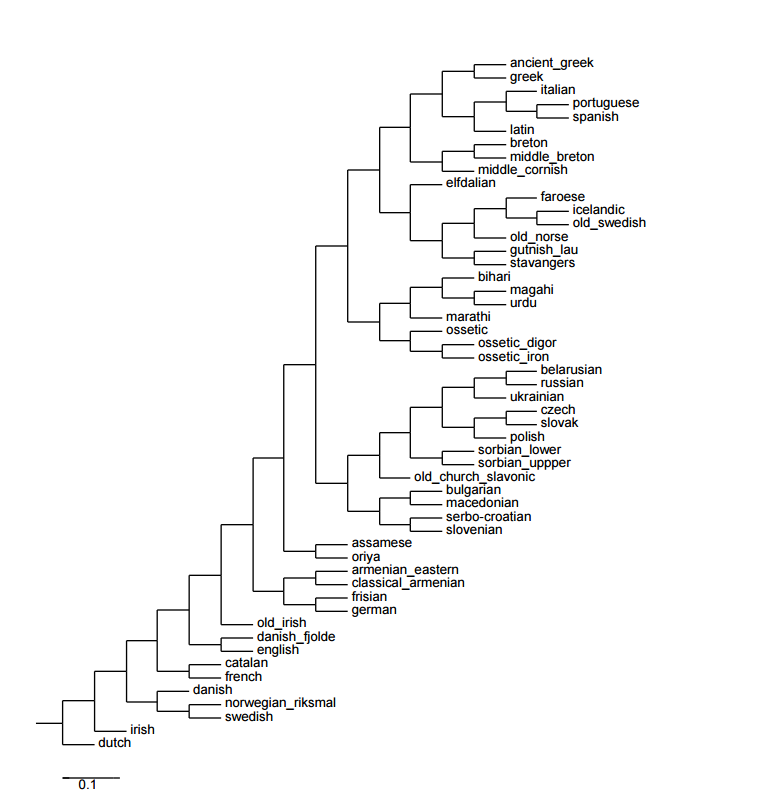
\includegraphics[width=\linewidth]{tree2(2)}
	\caption{Tree visualization of Rao-distance measurements}
	\label{fig:raotree}
\end{figure*}


\section{Discussion}

Overall, our results seem to reflect positively on the validity of the methodology.  It appears to group similar languages together by an objective measure of the language into generally well-accepted families.  Our results, however, seem weaker than those of Kirby and Ellison.

There are several routes that could be explored for improving the results.  We could have experimented more with how to handle meanings with multiple words, perhaps by taking the minimum confusion probability value or average of the values.  This likely would only have a minor influence on the results, but perhaps a noticeable impact.

The data may also have been lacking, given that so few of the word meanings were found in the data set for all languages.  A larger and more consistent spread of word meanings in the languages may have resulted in more representative lexical metrics and better comparisons between them for measuring distance.

Another avenue for improvement may lie in that our means of calculating edit distances between phonemic transcriptions was not as effective as using orthography, as such transcriptions are not consistent and can be difficult to get an accurate distance measurement out of.  Dealing with how these transcriptions were encoded and comparing them is also challenging, and we may have had better results using third-party libraries that handled this more effectively.  It may even be the case that orthography does a better job of comparing the relatedness of words than phonemic transcriptions, as the orthography could better capture the ancestry of the word.

\section{Conclusion}

This paper presented a reimplementation of an automatic language phylogeny constructing algorithm described by \citeA{ellison2006measuring}, which uses inter-language comparisons of words to build a lexical network that is compared against other languages, measuring their similarity.  This was conducted on a new data set, using phonemic transcriptions instead of orthography for comparing individual words.  We obtained encouraging results that seemed to group languages well, but the results were likely less strong than those from Kirby and Ellison.  Some possible explanations for this were identified, and opened paths for further exploration.


\bibliographystyle{apacite}

\setlength{\bibleftmargin}{.125in}
\setlength{\bibindent}{-\bibleftmargin}

\bibliography{LVC}


\end{document}
